\begin{figure}[h]
	\centering
	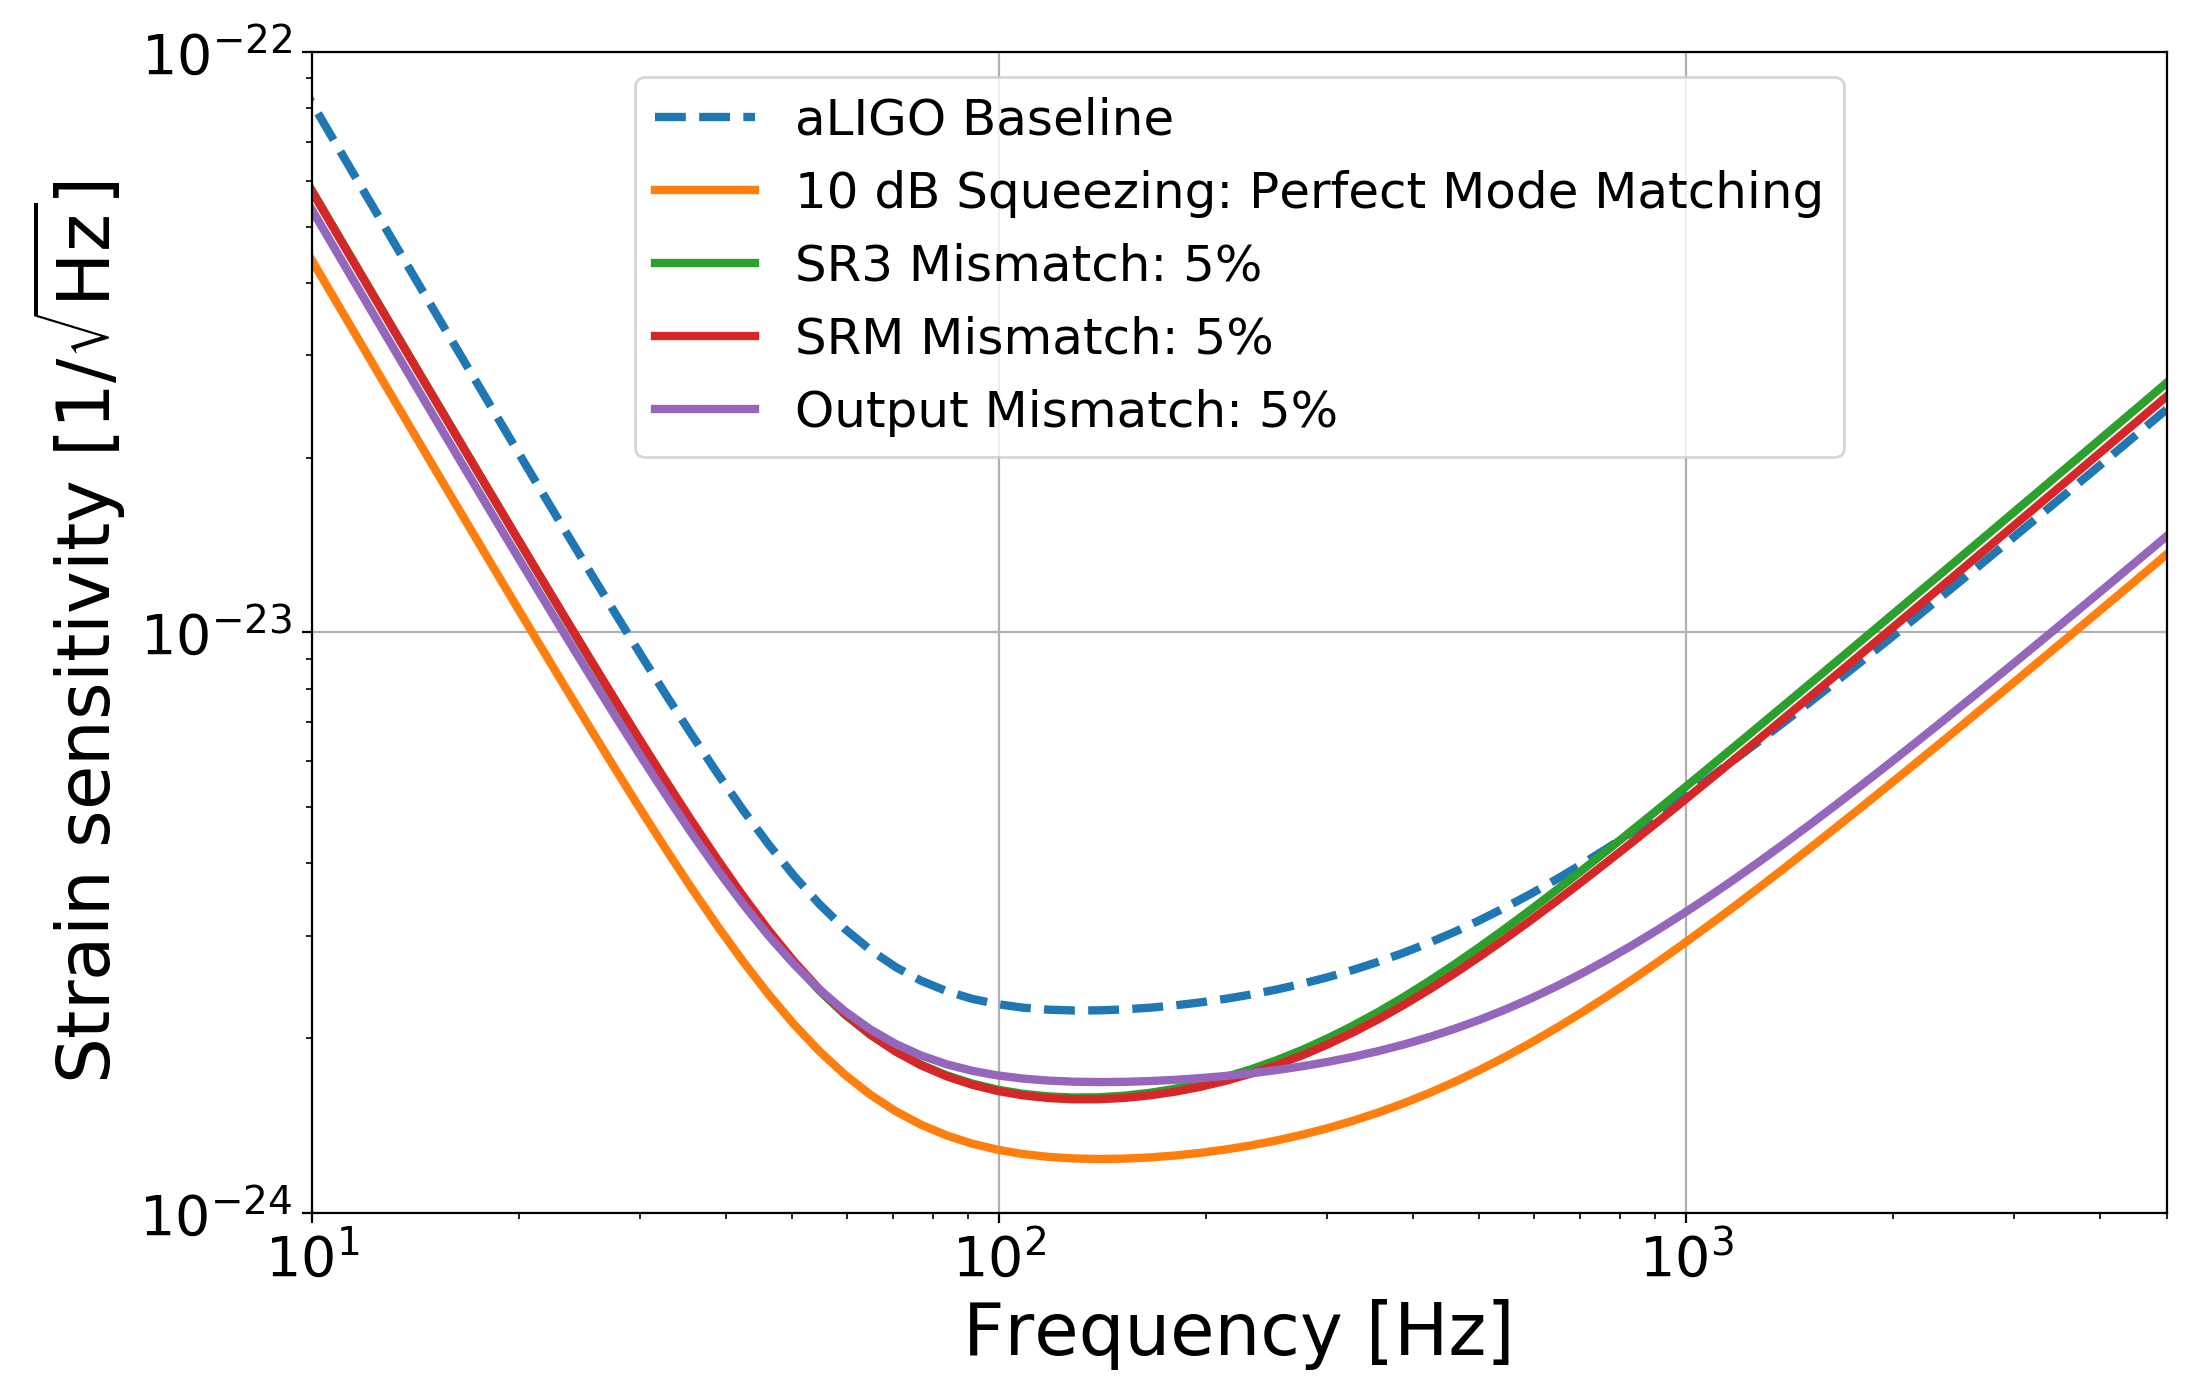
\includegraphics[width=1.0 \textwidth]{../Figures/QM_sens_compare_mismatches.png}
	\caption[Quantum limited sensitivity simulation to compare mismatches in the presence of squeezed light.]
	{\textbf{Quantum limited sensitivity simulation to compare mismatches in the presence of squeezed light.} 
		With 10 db of broadband squeezing, the simulation introduced mismatch at various actuators to change the mode shape at the output port.  Although there is still 5\% mismatch in each case, the introduction of quantum noise and the degradation of squeezing is much worse when introducing losses in the signal recycling cavity as opposed to the output train.  In addition, mismatching the signal recycling cavity will change the relative phase angle between the interferometer and squeezed light which has to be re-optimized.	
	}
	\label{fig:QM_lim_sens_mismatch}
\end{figure}

\begin{sidewaystable}
	\centering
\begin{tabular}{|l||r|r|r|r|r|r|r|r|}
	\hline
	 {} &     PRC w &    PRC S &     SRC w &    SRC S &    ARMs w &   ARMs S &   OMC w &     OMC S \\
	\hline
	\hline
PRM   &     4.537 &    0.006 &     0.000 &    0.000 &     0.000 &    0.000 &   0.000 &     0.000 \\
PR2   &   -45.004 &   -0.058 &     0.000 &    0.000 &     0.000 &    0.000 &   0.000 &     0.000 \\
PR3   & -3321.891 &   -4.315 &     0.000 &    0.000 &     0.000 &    0.000 &   0.000 &     0.000 \\
SRM   &     0.000 &    0.000 &    -5.097 &   -0.006 &     0.000 &    0.000 &   0.875 &     1.114 \\
SR2   &     0.000 &    0.000 &  -128.889 &   -0.160 &     0.000 &    0.000 &  -2.792 &   -99.513 \\
SR3   &     0.000 &    0.000 & -5460.964 &   -6.774 &     0.000 &    0.000 & -19.564 & -4294.447 \\
ITMTL & -3188.263 & 4142.666 & -5254.308 & 4140.289 &     0.000 & 	 0.000 &   0.000 &     0.000 \\
ITM   & -2310.433 & 3002.047 & -3807.633 & 3000.325 & -1827.435 & 3002.782 &   0.000 &     0.000 \\
ETM   &     0.000 &    0.000 &     0.000 &    0.000 &  3774.807 &    4.682 &   0.000 &     0.000 \\
OM1   &     0.000 &    0.000 &     0.000 &    0.000 &     0.000 &    0.000 &   0.164 &     0.552 \\
OM2   &     0.000 &    0.000 &     0.000 &    0.000 &     0.000 &    0.000 &   0.511 &    -0.889 \\
OM3   &     0.000 &    0.000 &     0.000 &    0.000 &     0.000 &    0.000 &  -0.222 &    -0.453 \\
	\hline
\end{tabular}
		\caption[Mode matching actuation matrix for the transverse x direction.]
	{\textbf{Mode matching actuation matrix for the transverse x direction.} Each of the row elements represent actuators and columns show the affected cavity defocus $S$ or beam size $w$ per diopter change, which are scaled by the initial perfect mode matching values.  For small mismatches, the slope is assumed to be linear.}
\label{tbl:x_act_matrix}
\end{sidewaystable}

\begin{sidewaystable}
	\centering
	\begin{tabular}{|l||r|r|r|r|r|r|r|r|}
		\hline
		{} &     PRC w &    PRC S &     SRC w &    SRC S &    ARMs w &   ARMs S &   OMC w &     OMC S \\
		\hline
		\hline
PRM   &     5.092 &    0.006 &     0.000 &    0.000 &     0.000 &    0.000 &   0.000 &     0.000 \\
PR2   &   -52.019 &   -0.062 &     0.000 &    0.000 &     0.000 &    0.000 &   0.000 &     0.000 \\
PR3   & -3852.041 &   -4.569 &     0.000 &    0.000 &     0.000 &    0.000 &   0.000 &     0.000 \\
SRM   &     0.000 &    0.000 &    -6.870 &   -0.007 &     0.000 &    0.000 &   0.870 &     1.105 \\
SR2   &     0.000 &    0.000 &  -178.704 &   -0.169 &     0.000 &    0.000 &  -2.783 &   -99.469 \\
SR3   &     0.000 &    0.000 & -7589.021 &   -7.189 &     0.000 &    0.000 & -19.509 & -4292.095 \\
ITMTL & -3700.089 & 4142.316 & -7309.182 & 4139.780 &     0.000 &    0.000 &   0.000 &     0.000 \\
ITM   & -2681.338 & 3001.794 & -5296.743 & 2999.956 & -1827.470 & 3002.700 &   0.000 &     0.000 \\
ETM   &     0.000 &    0.000 &     0.000 &    0.000 &  3774.854 &    4.697 &   0.000 &     0.000 \\
OM1   &     0.000 &    0.000 &     0.000 &    0.000 &     0.000 &    0.000 &   0.172 &     0.557 \\
OM2   &     0.000 &    0.000 &     0.000 &    0.000 &     0.000 &    0.000 &   0.508 &    -0.887 \\
OM3   &     0.000 &    0.000 &     0.000 &    0.000 &     0.000 &    0.000 &  -0.165 &    -0.344 \\
	\hline
\end{tabular}
		\caption[Mode matching actuation matrix for the transverse y direction.]
{\textbf{Mode matching actuation matrix for the transverse y direction.} }
\label{tbl:y_act_matrix}
\end{sidewaystable}

\begin{figure}[h]
	\centering
	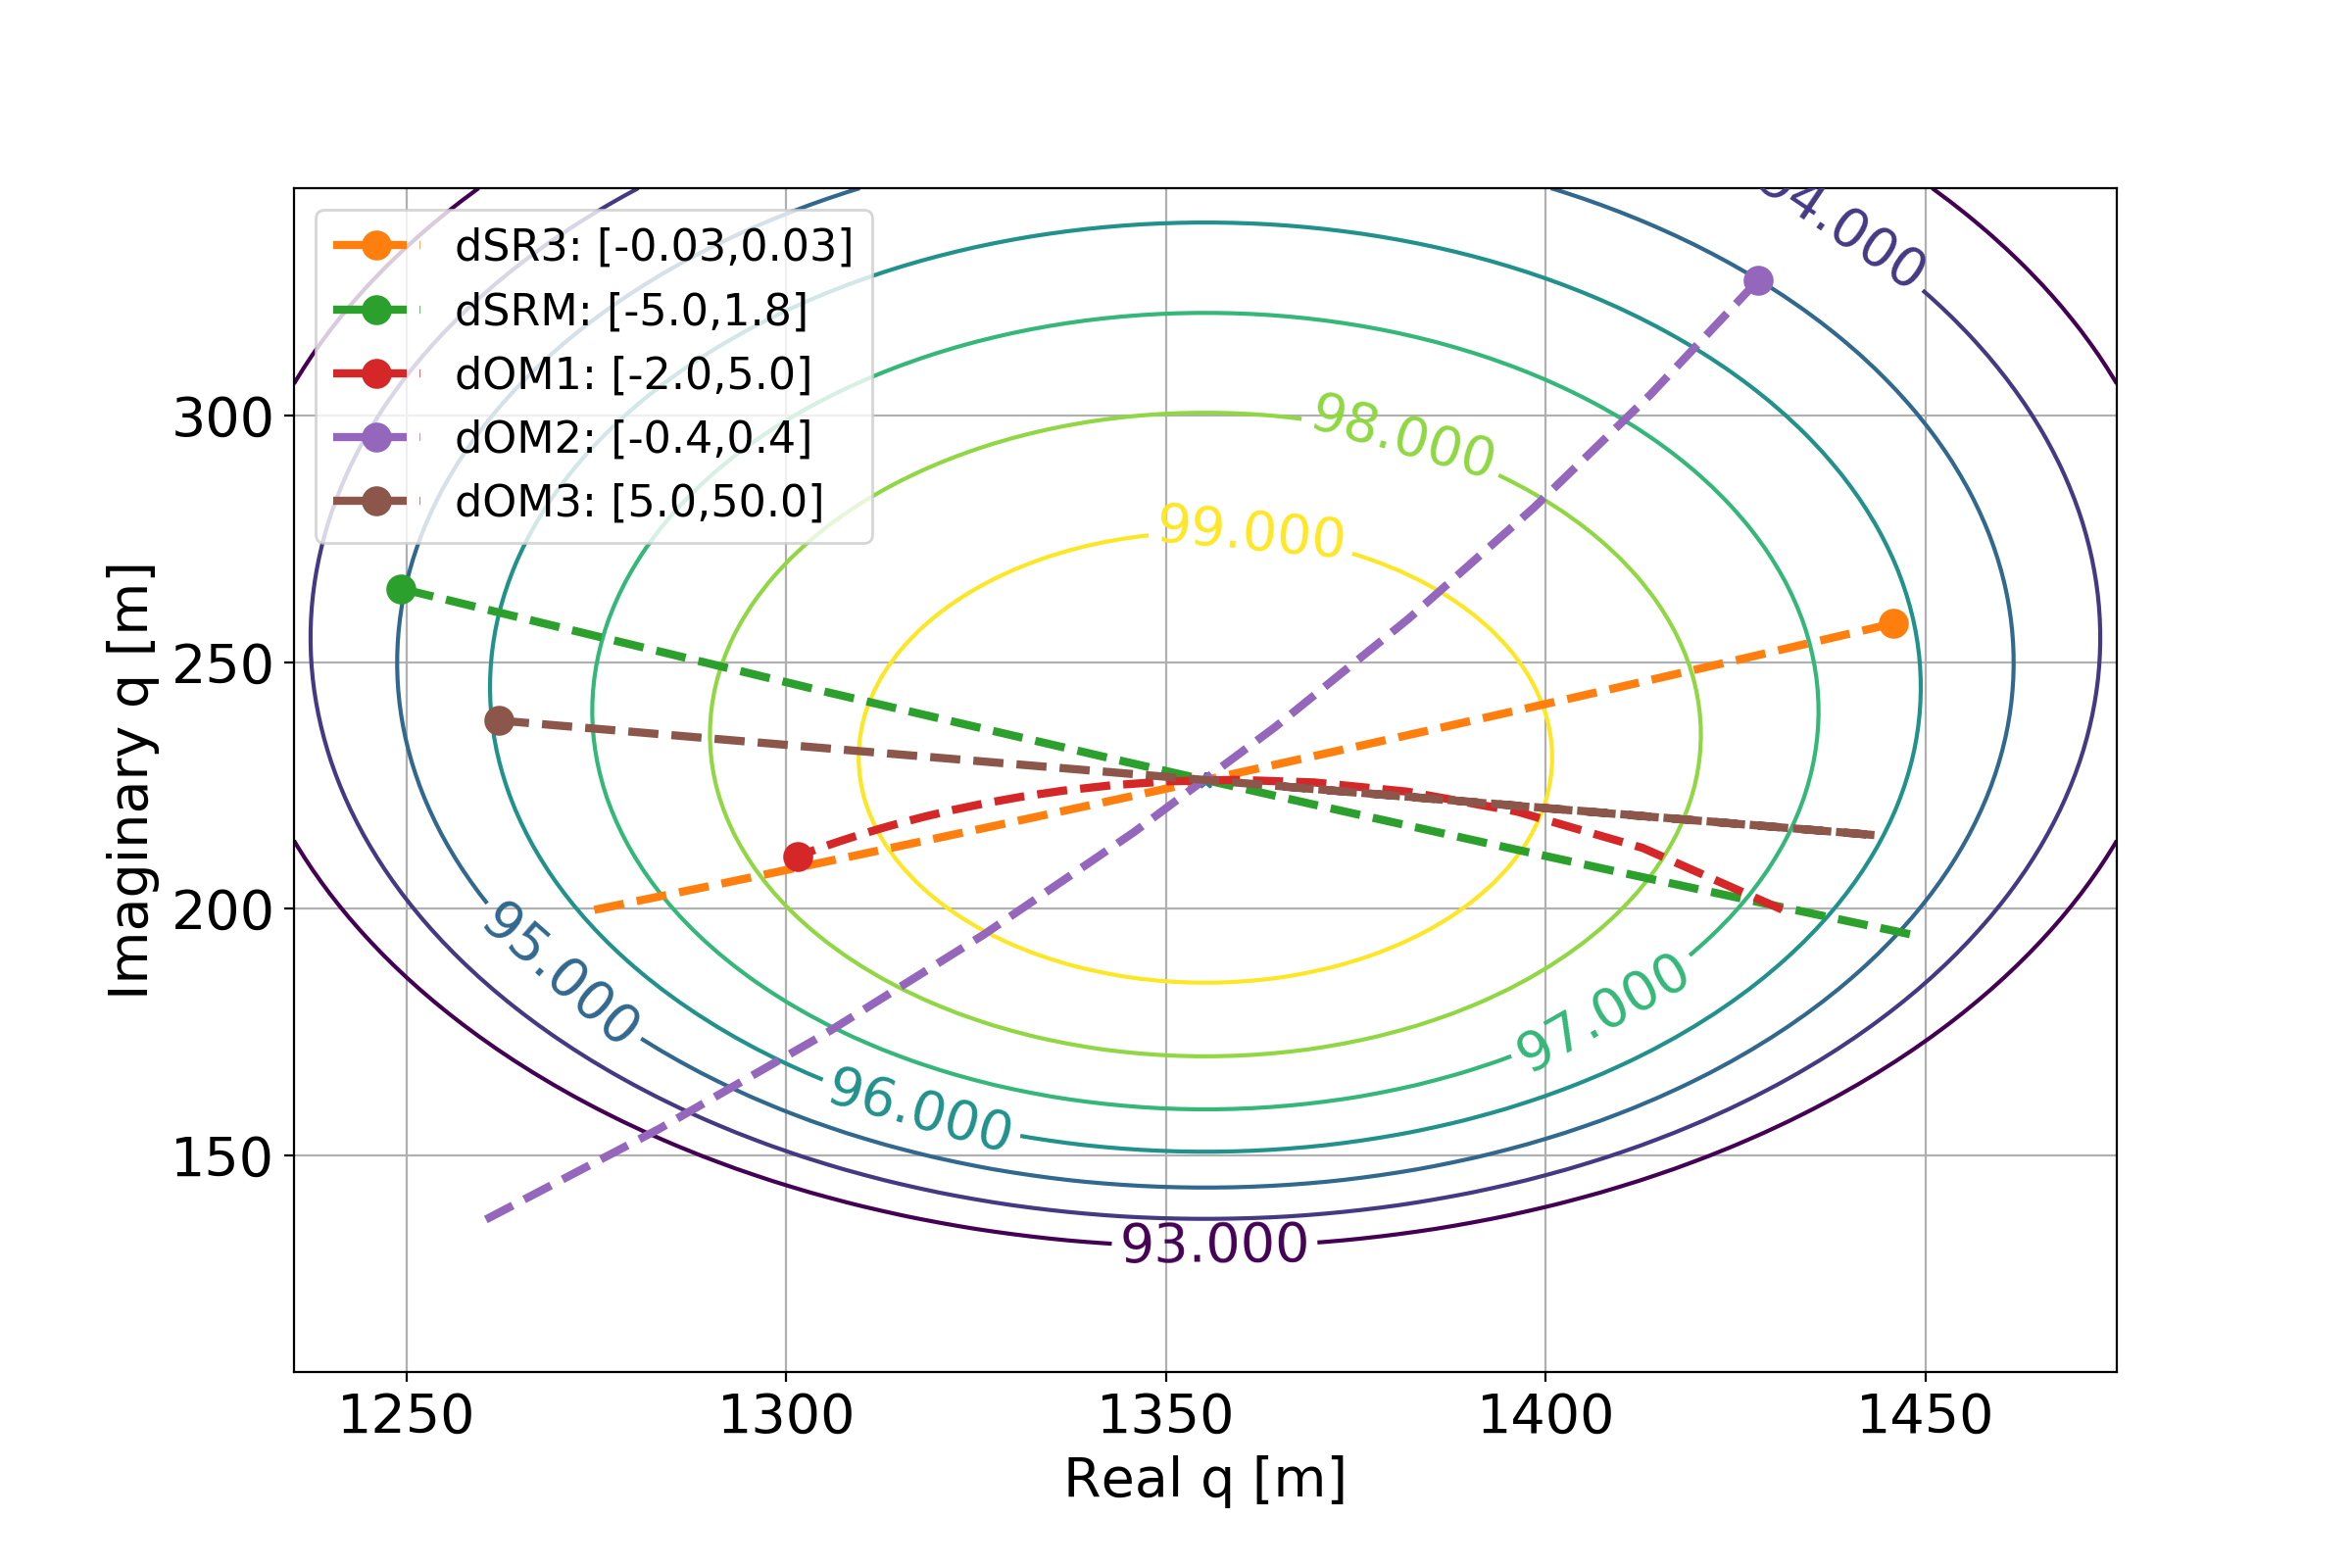
\includegraphics[width=1.0 \textwidth]{../Figures/OutputAct_Gouyphase.png}
	\caption[Simulating the output actuator phase spaces projected onto the OMC mode basis.]
	{\textbf{Simulating the output actuator phase spaces projected onto the OMC mode basis.} 
	By allowing FINESSE to do the ray tracing algorithm for the entire interferometer, it is relatively straightforward to change the radii of curvature for different optics and project the effect onto the OMC in order to understand the orthogonality when choosing mirrors for mode matching.  Interestingly, the most orthogonal actuators for small mismatches happen to be SRM and OM2, however, OM1 becomes quadratic much more quickly which leads to increased range.  The ending dots indicate the positive direction for changing radii of curvature as seen by the various optics.  Also, the change in radii of curvature in units of meters is shown on the legend.
	}
	\label{fig:act_phase_space}
\end{figure}

\begin{figure}[h]
	\centering
	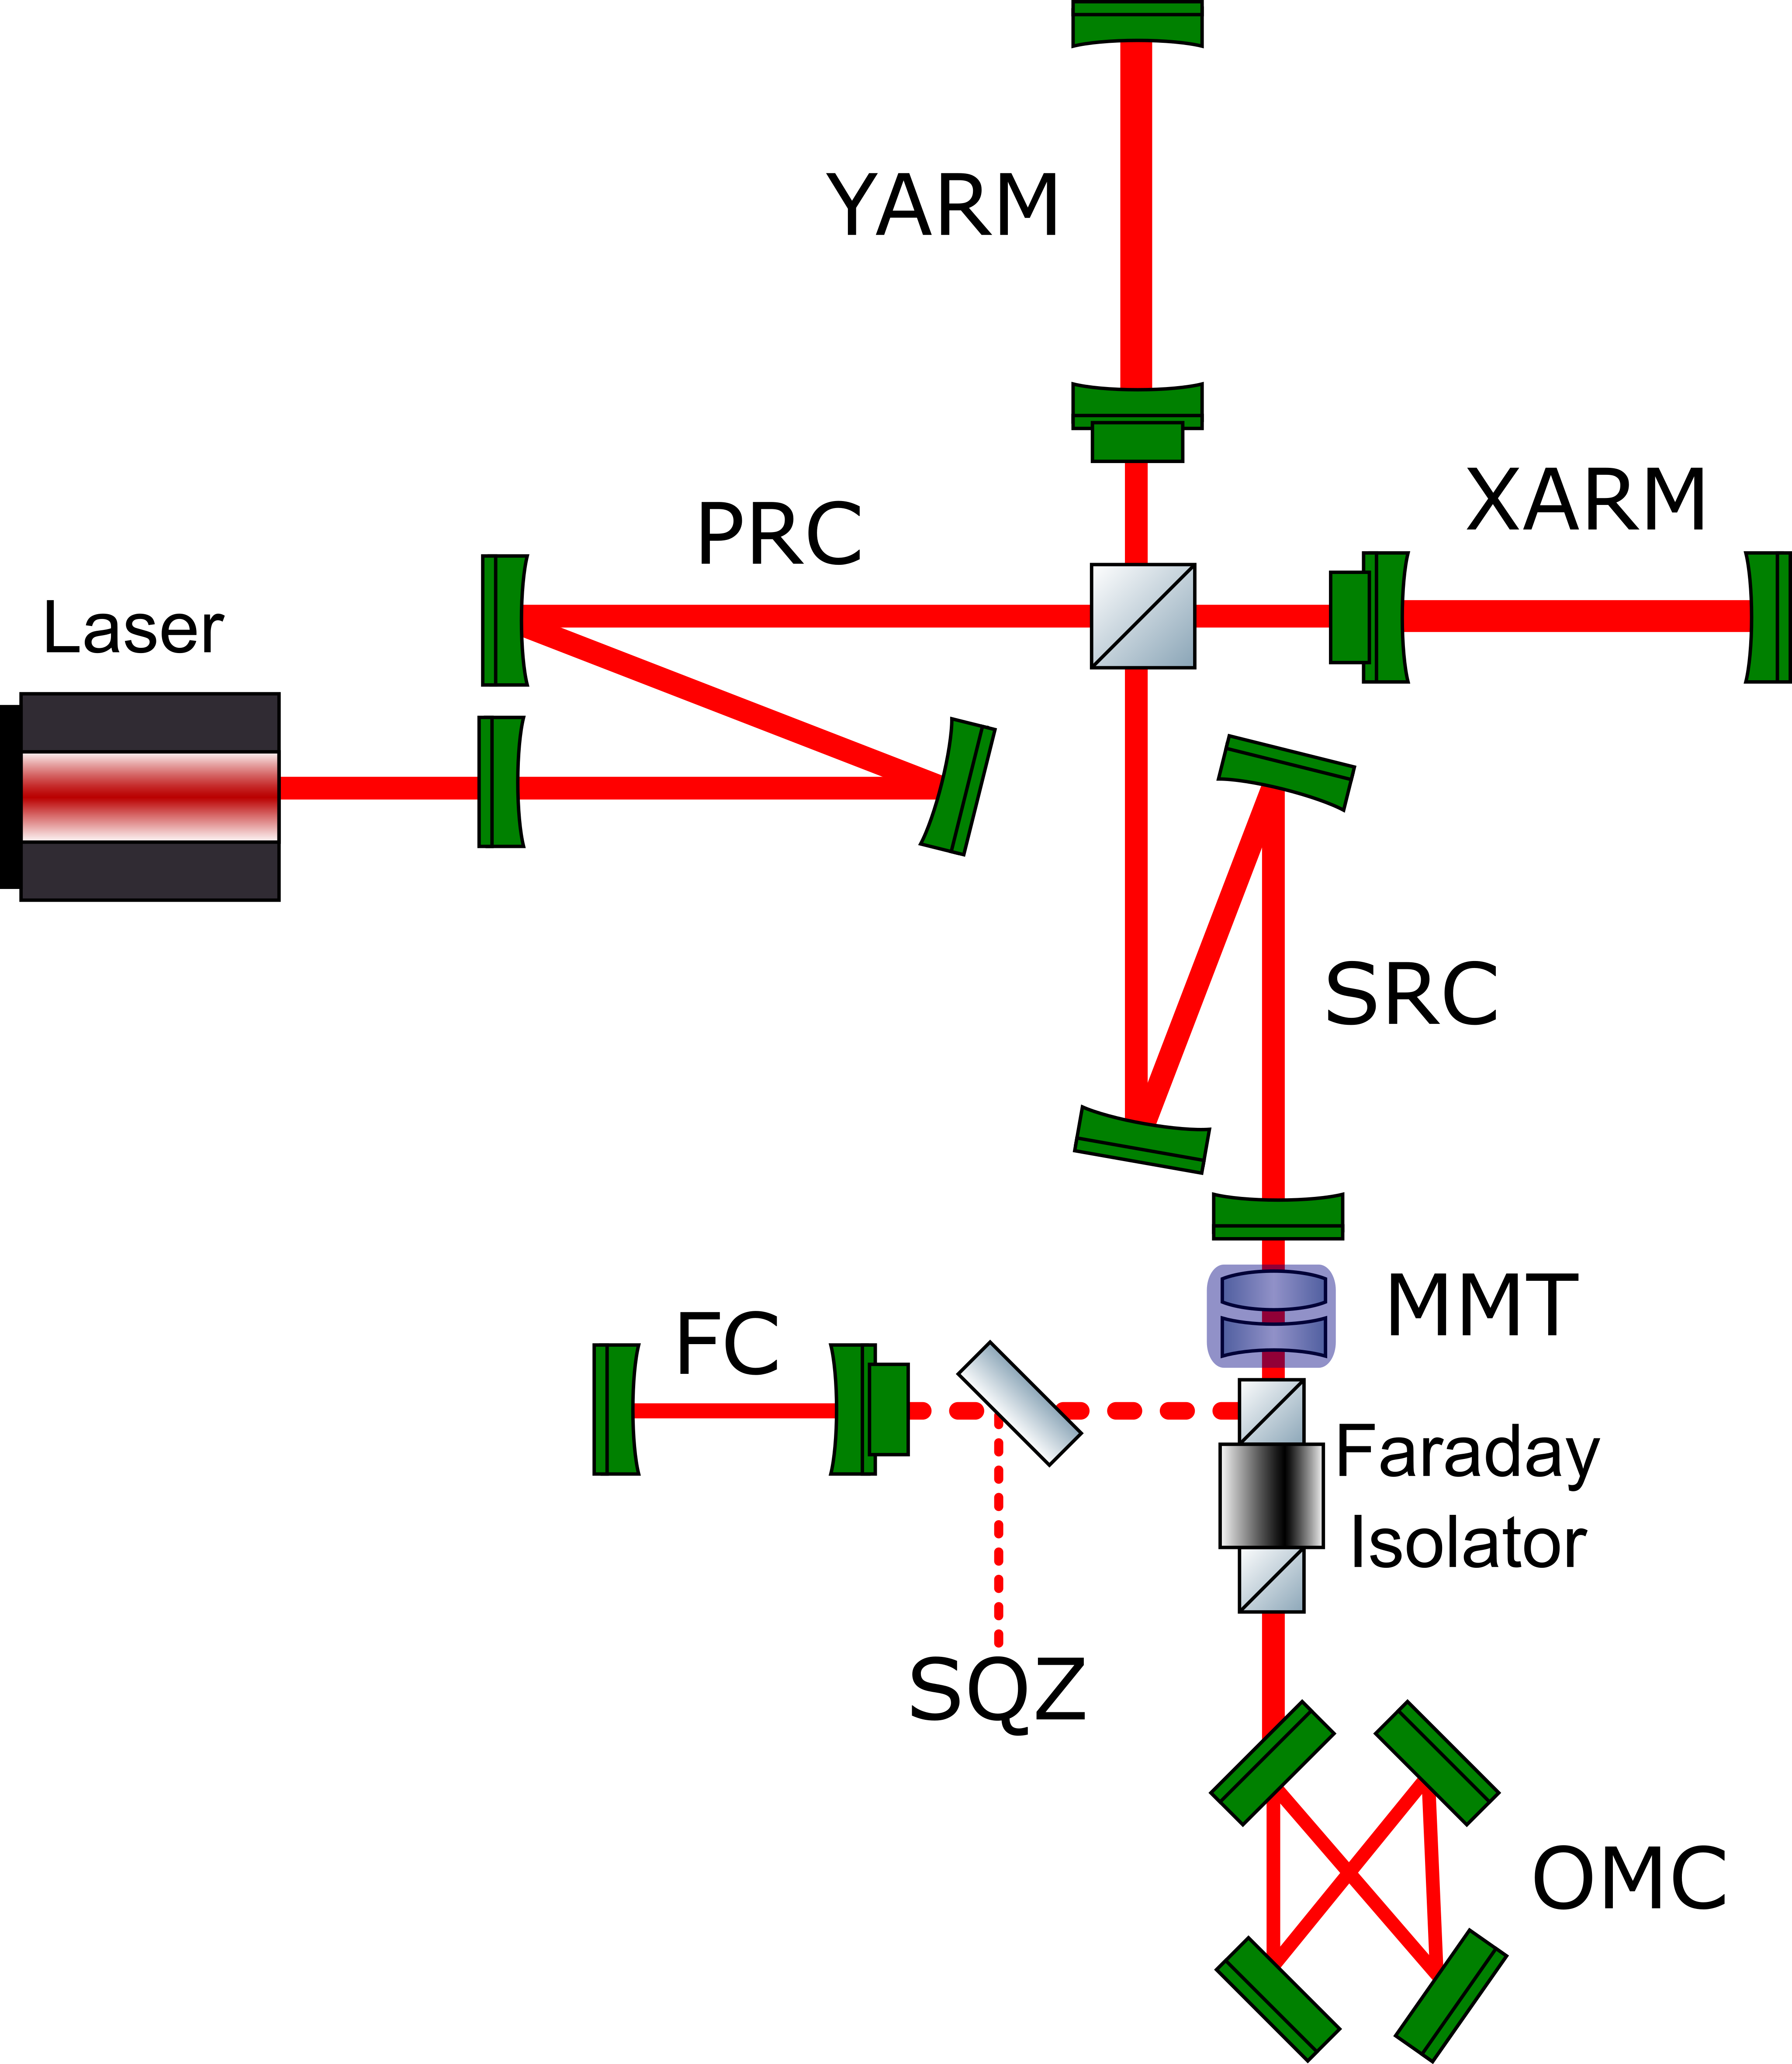
\includegraphics[width=0.8 \textwidth]{../Figures/FullIFO_FINESSE.png}
	\caption[Full interferometer simulation with FINESSE.]
	{\textbf{Full interferometer simulation with FINESSE.} 
		This includes squeezed light, a filter cavity, and an ideal mode matching telescope (highlighted in blue) at the signal recycling output port which can be turned on/off in order to understand the SRC mode mismatches without the lensing effects introduced when changing the SRM radius of curvature.
	}
	\label{fig:IFO_FINESSE}
\end{figure}

\begin{sidewaystable}
	\centering
\begin{tabular}{|l||r|r|r|r|r|r|r|r|}
\hline
	{Parameters} &      IMC &      XARM &      YARM &        PRX &        PRY &        SRX &        SRY &        OMC \\
\hline
\hline
Rayleigh Range [m]        &  13.338 &   427.807 &   427.807 &   5.314 &   5.314 &   2.132 &   2.132 &   0.708 \\
Waist to 1st Mirror [m]   & -16.473 & -1834.220 & -1834.220 &   6.940 &   6.940 &   4.733 &   4.733 &   0.141 \\
Cavity Length [m]      &  16.473 &  3994.500 &  3994.500 &  57.711 &  57.632 &  56.065 &  55.985 &   0.566 \\
FSR [MHz]                 &   9.099 &     0.038 &     0.038 &   2.597 &   2.601 &   2.674 &   2.677 & 264.975 \\
RT Gouy Phase [deg]       & 102.008 &   -48.661 &   -48.661 &  51.724 &  51.722 &  38.311 &  38.309 &  78.979 \\
Pole Frequency [kHz]      &   8.636 &     0.045 &     0.043 & 309.692 & 309.939 & 409.982 & 410.283 & 321.971 \\
Finesse                   & 526.837 &   413.523 &   436.867 &   4.193 &   4.196 &   3.261 &   3.263 & 411.488 \\
A                         &   1.000 &    -2.559 &    -2.559 &  -0.406 &  -0.406 &  -0.591 &  -0.591 &  -0.004 \\
B                         &  32.946 & -6225.726 & -6225.726 &  11.286 &  11.286 &   7.835 &   7.835 &   0.722 \\
C                         &  -0.073 &     0.002 &     0.002 &  -0.148 &  -0.148 &  -0.291 &  -0.291 &  -1.387 \\
D                         &  -1.416 &     3.880 &     3.880 &   1.645 &   1.645 &   2.161 &   2.161 &   0.386 \\
\hline
\end{tabular}
	\caption[Calculated cavity parameters for the advanced LIGO interferometer.]
	{\textbf{Calculated cavity parameters for the advanced LIGO interferometer.}
	The values were obtained using FINESSE's $cav$ commands which are an integral part of the beam tracing algorithm. Here, the power (and signal) recycling cavity is split into two linear resonators made up of the PRM and HR surface of the respective ITMs.  In an ideal world, the reflectivity of ITMX and ITMY are the same but can actually vary up to 5\% in the case of H1 \cite{galaxy}. This mostly affects the arm cavity Finesse but can have small effects on the power recycling cavity as well.}
	\label{tbl:cav_params}
\end{sidewaystable}
